
%%%%%%%%%%%%%%%%%%%%%%%%%%%%%%%%%%%%%%%%%%%%%%%%%%%%%%%%%%%%%%%%%%%%%%
%%%%                   Outcome
%%%%%%%%%%%%%%%%%%%%%%%%%%%%%%%%%%%%%%%%%%%%%%%%%%%%%%%%%%%%%%%%%%%%%%
\color{green}
\subsection{Glyph: \glyph{Outcome}}\label{sec:outcome}

\subsubsection{Introduction}

In \ER, an \glyph{outcome} represents the result of an \glyph{interaction} (section \ref{sec:interaction}) or an \glyph{assignment} (\ref{sec:assignment}). For instance, if an \glyph{interaction} represents a non-covalent binding, the \glyph{outcome} represents the complex. If an \glyph{interaction} represents a genetic interaction, for instance derived from genetic screenings, the \glyph{outcome} represents the result of the presence of the two polymorphisms. If an \glyph{assignment} represents the phosphorylation of a protein, the \glyph{outcome} represents the phosphorylated form of this protein.

\begin{glyphDescription}

\glyphSboTerm SBO:0000409 ! interaction outcome

\glyphContainer  An \glyph{outcome} is represented by a black dot located on the arc of an \glyph{interaction} (see section~\ref{sec:interaction}) or an \glyph{assignment} (see section~\ref{sec:assignment}). The diameter of the dot has to be larger than the thickness of the arc.

\glyphLabel An \glyph{outcome} has no identity on its own and does not carry any label. 

\glyphAux An \glyph{outcome} does not carry any auxiliary items.

\end{glyphDescription}

\begin{figure}[H]
  \centering
  \includegraphics[scale = 0.3]{images/outcome}
  \caption{The \ER glyph for \glyph{outcome}.}
  \label{fig:outcome}
\end{figure}

\normalcolor
	
